\section{Results}\label{sec:results}
% Built from the same scoped evidence as Supplement Table S1.
\begin{table}[tb]
\centering
\caption{Five achievements, original law. $\checkmark$ supported; $\times$ not supported; – not established: available evidence does not establish this achievement. Fractions are seeds passing out of three, except recoverability: supported slots out of five in seed order 0/1/2. Access: $D$ by design (exact sums supplied); $I$ demonstrated by a matched connection intervention. Complete scope, counts and controls: Supplement Table S1.}\label{tab:table1}
\begingroup\fontsize{8}{9.5}\selectfont\setlength{\tabcolsep}{3pt}\emergencystretch=1em\hyphenpenalty=10000\exhyphenpenalty=10000
\begin{tabular}{@{}>{\raggedright\arraybackslash}p{2.500in}>{\raggedright\arraybackslash}p{0.910in}>{\raggedright\arraybackslash}p{0.780in}>{\raggedright\arraybackslash}p{0.430in}>{\raggedright\arraybackslash}p{0.720in}>{\raggedright\arraybackslash}p{0.740in}@{}}
\toprule
\textbf{condition} & \textbf{recoverability} & \textbf{computation} & \textbf{access} & \textbf{preservation} & \textbf{reliable prediction} \\
\midrule
r8: records $\to$ prediction & $\checkmark$ 1/5$\cdot$1/5$\cdot$1/5 & – & – & – & $\times$ 0/3 \\
r10: records $\to$ prediction & $\checkmark$ 5/5$\cdot$5/5$\cdot$5/5 & – & – & – & $\times$ 0/3 \\
r10: records $\to$ prediction+sums & $\checkmark$ 5/5$\cdot$5/5$\cdot$5/5 & – & – & – & $\times$ 0/3 \\
r11: records $\to$ prediction (Erosion continuation) & $\checkmark$ 1/5$\cdot$1/5$\cdot$1/5 & $\times$ 0/3 & – & $\times$ & $\times$ 0/3 \\
r11: records $\to$ prediction+sums (Erosion continuation) & $\checkmark$ 3/5$\cdot$1/5$\cdot$1/5 & $\checkmark$ 1/3 & – & $\times$ & $\checkmark$ 1/3 \\
r12: records $\to$ prediction+sums & $\checkmark$ 5/5$\cdot$5/5$\cdot$5/5 & $\times$ 0/3 & – & – & $\times$ 0/3 \\
r12: records+sums $\to$ prediction & $\checkmark$ 2/5$\cdot$2/5$\cdot$3/5 & $\checkmark$ 3/3 & $\checkmark^{D}$ & $\checkmark^{f}$ & $\checkmark$ 2/3 \\
r13: records $\to$ prediction+sums & – & $\times$ 0/3 & – & – & $\times$ 0/3 \\
r13: Connected (frozen) & – & $\times$ 0/3 & $\checkmark^{I}$ & $\checkmark^{f}$ & $\times$ 0/3 \\
r13: Connected (live) & – & $\times$ 0/3 & $\checkmark^{I}$ & – & $\times$ 0/3 \\
r13: records+sums $\to$ prediction (exact supplied) & – & $\checkmark$ 3/3 & $\checkmark^{D}$ & $\checkmark^{f}$ & $\checkmark$ 1/3 \\
r13: records+sums $\to$ prediction (Numerical encoding) & – & $\checkmark$ 3/3 & $\checkmark^{D}$ & $\checkmark^{f}$ & $\times$ 0/3 \\
r13: blocked prediction gradient & – & $\checkmark$ $3/3^{\ell}$ & – & $\checkmark^{b}$ & – \\
\bottomrule
\end{tabular}
\par\smallskip
\begin{minipage}{\textwidth}\textit{Note.} Raw-carrier linear readers: 512 held-out boards/slot. Computation: the audited sums output, exact vectors on rendering 0 (24,435 boards); $\ell$: 1,555 local histories. The connection intervention does not establish selective use. $f$: frozen supplier; $b$: blocked-gradient control. Frozen preservation is design-limited.\end{minipage}
\endgroup
\end{table}


\Cref{tab:table1} summarizes, for each version and condition, which of the
five achievements of realizing the designed decomposition the evidence
supports; its columns follow the order used throughout (recoverability, computation, access,
preservation, reliable prediction). Unless stated otherwise, results
use the original law, the 20,000-update endpoint and census rendering~0,
and values are per seed in seed order (0 / 1 / 2).

\subsection{Training shapes what becomes recoverable}\label{sec:res-recover}
\begin{figure}[tb]
\centering
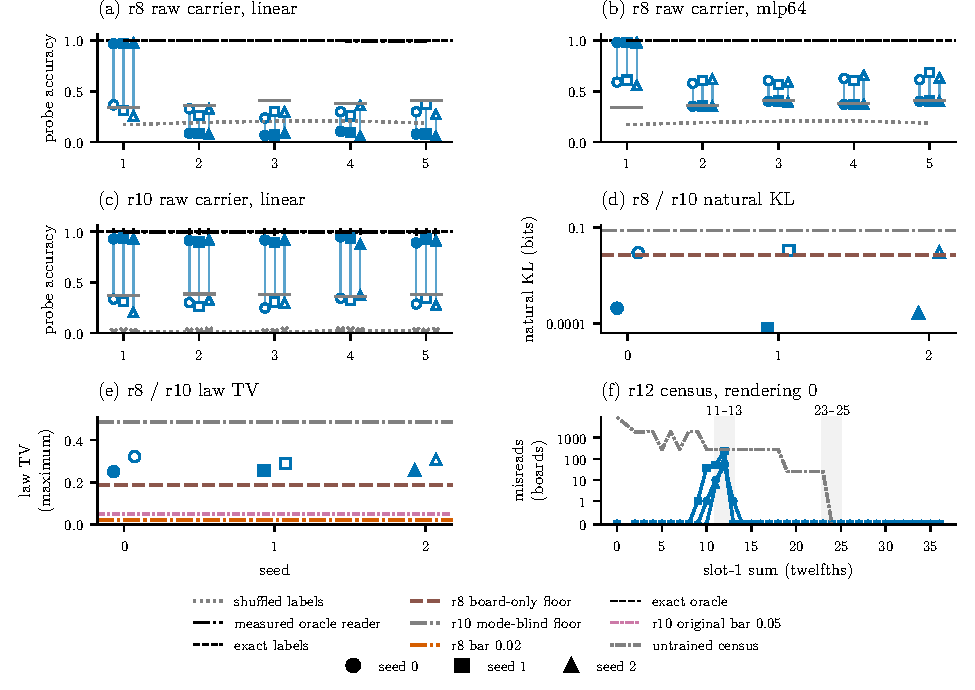
\includegraphics[width=\textwidth]{figures/fig3.pdf}
\caption{\csname captionfig3\endcsname}\label{fig:fig3}
\end{figure}


\textbf{Claim: training on B gives the network a jagged version of A,
readable where B needs it and less readable where it does not.} In the
records $\to$ prediction networks of r8, a linear probe on the raw carrier
recovers the slot-1 sum on 97--98\% of held-out boards at the endpoint, up
from 26--37\% at update~0 (ranges over three seeds; \cref{fig:fig3}a). The sums of slots 2--5, which
the prediction never needs, become \emph{less} readable: from 24--37\% at
update~0 (mean 30\%) to 5--10\% at the endpoint (ranges over four slots
and three seeds). A one-hidden-layer probe shows the same
direction (about 60\% to 38\%, mean over slots 2--5 and three seeds;
\cref{fig:fig3}b). The linear probe weights classes equally, so part of the
drop below the majority floor reflects that weighting; we read the decline as
reduced measured readability, not as removal of information. In the
all-slots task (r10), where the law depends on whichever slot is queried,
linear probes on the raw carrier recover all five sums: 20--37\% at
update~0 and 88--95\% at the endpoint over five slots and three seeds, with
every paired 95\% gain interval above zero (\cref{fig:fig3}c).

\emph{Scope.} The r8--r10 comparison is historical and crosses tasks. It
supports task-dependent organization of what is recoverable, not exact
computation or use; rare r10 sum values (28--36) lie outside the registered
scope.

\subsection{Average error hides specific failures}\label{sec:res-average}

\textbf{Claim: B combines low average error with category misreads
concentrated near the slot-1 cutoffs and failures on particular histories.}
The r8 records $\to$ prediction networks reach a natural KL of
0.00030 / 0.00007 / 0.00021 bits, far below the 0.01 bar and the board-only
predictor's 0.0135 bits (\cref{fig:fig3}d). Yet none of the three runs
passes: on the constructed law panels the maximum law TV is
0.250 / 0.255 / 0.256, worse than the board-only predictor (0.188) and
twelve times the 0.02 bar (\cref{fig:fig3}e). A separate census of the r12 records $\to$ prediction networks (uniform
sampling) locates the board failures: 57 of 58, 289 of 328 and 87 of 87
categorical misreads lie in the cutoff band; the rest lie at slot-1 sums 9
and 10, just below it (\cref{fig:fig3}f).

One might expect training on long histories to remove the history
failures. r12 added history coverage, and its long-panel errors are smaller
than r11's (a historical comparison: curriculum and loss weighting also
changed). Even so, none of the nine
r12 records $\to$ prediction runs passes (three board-sampling arms $\times$
three seeds).
Long-panel maxima reach 0.172 and short-panel maxima range 0.020--0.066. We
diagnosed 162 selected histories from these runs. 120 stay within the
diagnostic 0.02-TV bar. Of the remaining 42, 20 are board-associated (all
coincident with a misread of the current board), 3 are
recurrence-associated, and 19 are unresolved. Misreads therefore do not
account for every failure.
Enriching training with boards at the cutoff values (r11) did not repair the
misreads consistently across seeds (\cref{app:tables}).

\subsection{Target noise contributes but is not sufficient}\label{sec:res-noise}
\begin{figure}[tb]
\centering
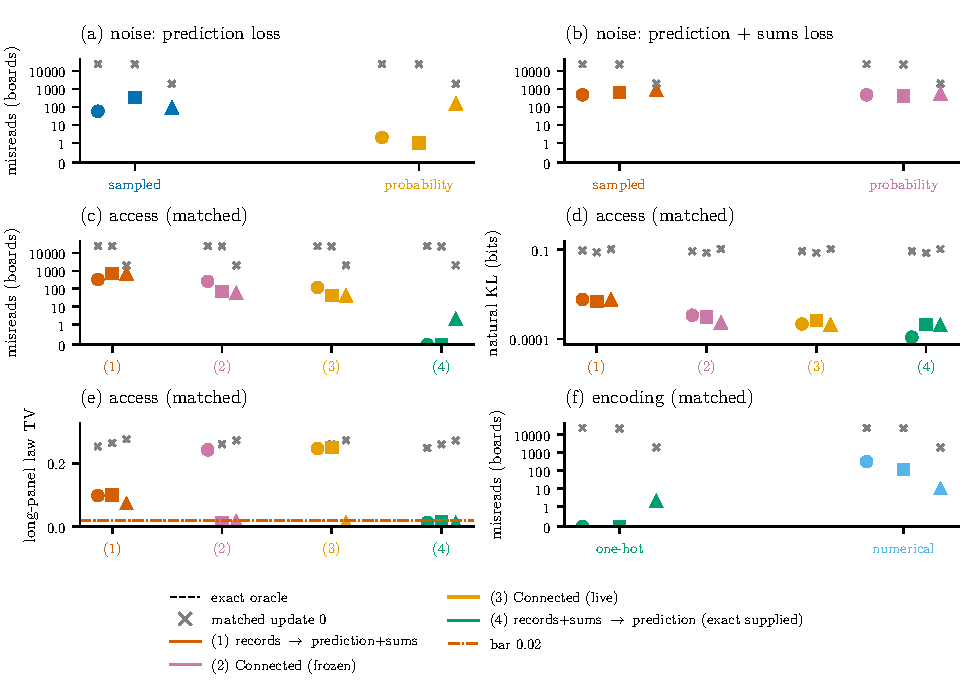
\includegraphics[width=\textwidth]{figures/fig4.pdf}
\caption{\csname captionfig4\endcsname}\label{fig:fig4}
\end{figure}


\textbf{Claim: the noise of sampled targets is one contributing condition.}
In this matched r13 comparison, training on the exact law instead of one
sampled next category removes target noise and changes nothing else. For records $\to$ prediction, census misreads
go from 58 / 328 / 87 with sampled targets to 2 / 1 / 149 with probability
targets: two seeds fall to near zero and the third gets worse
(\cref{fig:fig4}a). For records $\to$ prediction+sums they go from
473 / 648 / 815 to 473 / 400 / 523 (\cref{fig:fig4}b). No run passes under
either target. Removing target noise neither repairs every seed nor produces a pass.

\subsection{Computing or recovering the sums does not guarantee access}\label{sec:res-access}

\textbf{Claim: a network can produce the sums largely correctly, or hold them
in recoverable form, and still not deliver them to the prediction; access is
a separate achievement.}

\emph{Supplied versus learned sums (r12, matched versions).} In r12, the matched
comparison of the declared versions differs in three ways at once: whether
exact sums are supplied, how accurate the sums are, and whether the sums
are supervised. The records+sums $\to$ prediction
networks, which receive exact sums, pass 2 of 3 runs with 0--1 misreads. The
records $\to$ prediction+sums networks, which are trained to output the sums
but do not feed them to the prediction, pass 0 of 3 with 473--815 misreads.
Among boards where their own sums output gets the slot-1 category right,
their prediction still has a categorical misread on 326 / 617 / 770. Their sums output is
correct on 19,269 / 20,516 / 19,544 of the 24,435 completed sum boards, so
these networks compute the sums largely but not exactly. The comparison
supports more reliable prediction with exact supplied sums under these
conditions; it does not isolate access.

\emph{Connection (r13, matched).} The direct test of access is r13's
connection experiment, which connects the learned sums output to the
prediction and changes nothing else (\cref{fig:fig4}c--e). Relative to the
disconnected networks (331 / 725 / 637 misreads), Connected (frozen) has
259 / 69 / 58 misreads, a 1.3--11-fold reduction, and Connected (live) has
117 / 43 / 39, a 2.8--17-fold reduction. Natural KL falls as well, from
0.0018--0.0021 bits to 0.0003--0.0006 bits. Access does not by itself produce reliable prediction: no connected run passes every criterion,
and long-history failures can remain (Connected (live), seed 1: long-panel
maximum 0.251). This supports access as a cause of the misread reduction,
not a selective internal representation of the sums.

\emph{Swap test (r10).} In r10, probes recover all five sums and the swap
test passed calibration,
but on the trained networks the tested alignment was not selective: 188--436
of 1,024 swaps changed another slot's decoded sum. The failed selectivity means only that this test cannot support use under
this alignment.

\subsection{The form of access matters}\label{sec:res-encoding}
\begin{figure}[tb]
\centering
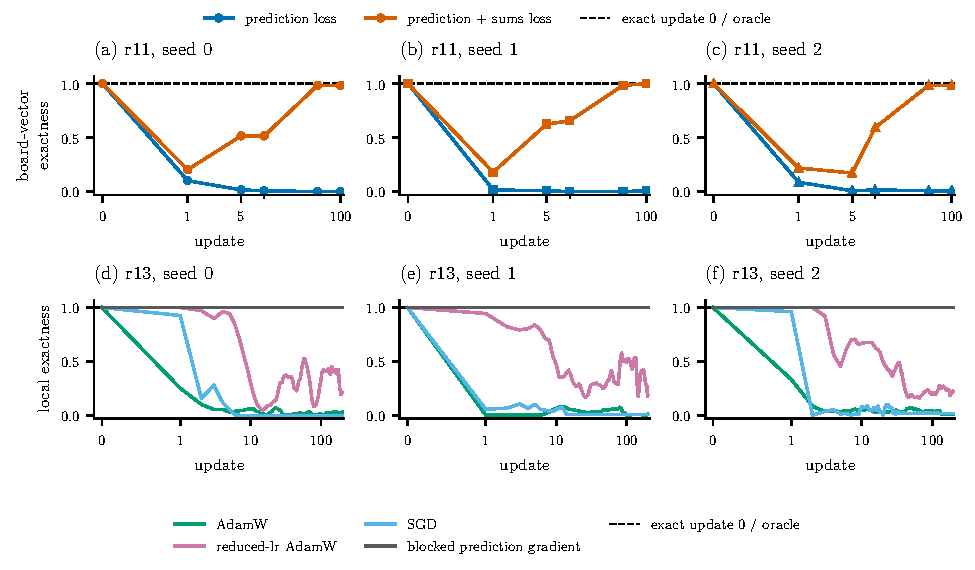
\includegraphics[width=\textwidth]{figures/fig5.pdf}
\caption{\csname captionfig5\endcsname}\label{fig:fig5}
\end{figure}


\textbf{Claim: the same exact information can be easy or hard to use,
depending on how it is encoded.} Given the same exact sums, the one-hot
encoding gives 0 / 0 / 2 misreads and the numerical encoding
$(s/36,\,1-s/36)$ gives 317 / 121 / 10 (\cref{fig:fig4}f). The two
conditions differ only in the encoding. A candidate reason, which these runs
do not test, is that a numerical input requires the prediction to place a
threshold between adjacent values such as 12 and 13 twelfths, whereas a
one-hot input gives each value its own input unit. A supplementary probe analysis of the cutoff values is in
\cref{app:probes}. We do not infer a precision ceiling from these results.

\subsection{Prediction updates erode an exact sums computation}\label{sec:res-erosion}

\textbf{Claim: a computation that is exact can be lost when training
continues on the prediction alone; preservation is a separate achievement.}
In r11, training continued from an exact sums network. With the prediction
loss only, board-vector exactness on a fixed panel of 128 boards falls from
1.0 at update~0 to 13/128, 2/128 and 11/128 at update~1 and remains
severely degraded at later sampled readouts
(\cref{fig:fig5}a--c). Keeping the sums loss largely protects the
computation, though not everywhere: at the endpoint, 24,434 / 24,435 /
24,419 of the 24,435 completed sum boards are correct.

r13 measured the first 200 updates exhaustively on the 1,555 local
histories (\cref{fig:fig5}d--f). Exactness is lost at update~1 under every
tested active optimizer, with very different severity. After one update,
AdamW keeps 393 / 5 / 518 histories exact, AdamW with a tenfold smaller
learning rate keeps 1,554 / 1,468 / 1,553, and SGD keeps 1,440 / 89 / 1,495.
When the prediction gradient to the sums network is blocked and weight decay
continues, all 1,555 histories stay exact through 200 updates in every seed.
Within the range of cumulative movement that all three optimizers covered,
exactness falls for each (\cref{fig:appendix_D_movement}). Erosion is therefore not
specific to Adam. These runs do not separate the direction of the prediction
gradient, the size of the displacement and the margins of the sums answers
as causes.

\subsection{Correct sums do not guarantee reliable prediction}\label{sec:res-reliable}

\textbf{Claim: even with exact sums supplied, reliable prediction is a
further achievement that some seeds miss.} With exact sums supplied as
input, r8's records+sums $\to$ prediction passes 3 of 3 runs, and records+sums $\to$ prediction (sums route only) passes 2 of 3. r12's records+sums $\to$
prediction passes 2 of 3, and r13's one-hot exact condition passes 1 of 3
(\cref{tab:table2}). In the all-slots task (r10), with its own criteria, the
version given exact sums passes 0 of 3. These are historical
comparisons across studies with different training protocols. A pass is also
not exhaustive correctness: the passing r13 seed still misreads 2 boards in
the census. The failed criteria of the supplied-sums networks are specific: r12 seed~2
exceeds the bar on the reset swap (TV 0.0590), r13 seed~0 on the single
\Lcat{} history (law TV 0.02275), and r13 seed~1 on the neutral swap (TV
0.02067). The sums are exact in all of them; candidates include the history update, the probability readout and the
response to interventions. We have not identified their mechanisms.
